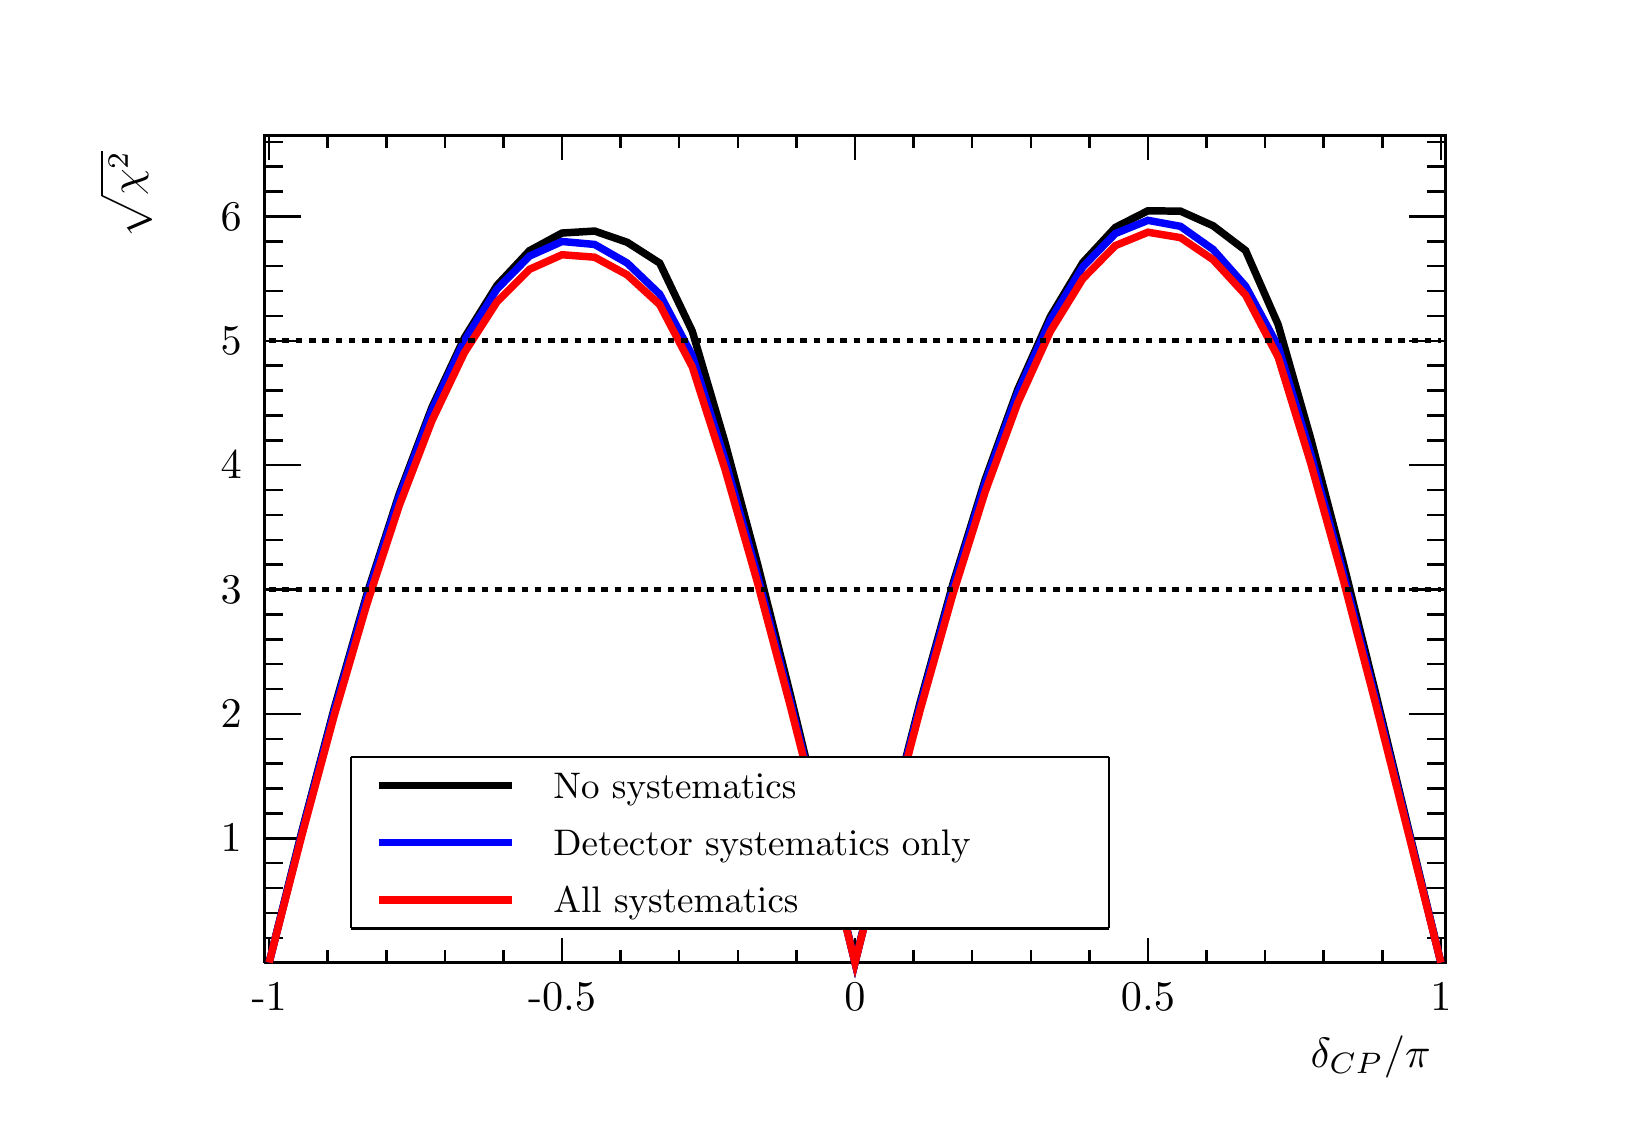
\begin{tikzpicture}
\pgfdeclareplotmark{cross} {
\pgfpathmoveto{\pgfpoint{-0.3\pgfplotmarksize}{\pgfplotmarksize}}
\pgfpathlineto{\pgfpoint{+0.3\pgfplotmarksize}{\pgfplotmarksize}}
\pgfpathlineto{\pgfpoint{+0.3\pgfplotmarksize}{0.3\pgfplotmarksize}}
\pgfpathlineto{\pgfpoint{+1\pgfplotmarksize}{0.3\pgfplotmarksize}}
\pgfpathlineto{\pgfpoint{+1\pgfplotmarksize}{-0.3\pgfplotmarksize}}
\pgfpathlineto{\pgfpoint{+0.3\pgfplotmarksize}{-0.3\pgfplotmarksize}}
\pgfpathlineto{\pgfpoint{+0.3\pgfplotmarksize}{-1.\pgfplotmarksize}}
\pgfpathlineto{\pgfpoint{-0.3\pgfplotmarksize}{-1.\pgfplotmarksize}}
\pgfpathlineto{\pgfpoint{-0.3\pgfplotmarksize}{-0.3\pgfplotmarksize}}
\pgfpathlineto{\pgfpoint{-1.\pgfplotmarksize}{-0.3\pgfplotmarksize}}
\pgfpathlineto{\pgfpoint{-1.\pgfplotmarksize}{0.3\pgfplotmarksize}}
\pgfpathlineto{\pgfpoint{-0.3\pgfplotmarksize}{0.3\pgfplotmarksize}}
\pgfpathclose
\pgfusepathqstroke
}
\pgfdeclareplotmark{cross*} {
\pgfpathmoveto{\pgfpoint{-0.3\pgfplotmarksize}{\pgfplotmarksize}}
\pgfpathlineto{\pgfpoint{+0.3\pgfplotmarksize}{\pgfplotmarksize}}
\pgfpathlineto{\pgfpoint{+0.3\pgfplotmarksize}{0.3\pgfplotmarksize}}
\pgfpathlineto{\pgfpoint{+1\pgfplotmarksize}{0.3\pgfplotmarksize}}
\pgfpathlineto{\pgfpoint{+1\pgfplotmarksize}{-0.3\pgfplotmarksize}}
\pgfpathlineto{\pgfpoint{+0.3\pgfplotmarksize}{-0.3\pgfplotmarksize}}
\pgfpathlineto{\pgfpoint{+0.3\pgfplotmarksize}{-1.\pgfplotmarksize}}
\pgfpathlineto{\pgfpoint{-0.3\pgfplotmarksize}{-1.\pgfplotmarksize}}
\pgfpathlineto{\pgfpoint{-0.3\pgfplotmarksize}{-0.3\pgfplotmarksize}}
\pgfpathlineto{\pgfpoint{-1.\pgfplotmarksize}{-0.3\pgfplotmarksize}}
\pgfpathlineto{\pgfpoint{-1.\pgfplotmarksize}{0.3\pgfplotmarksize}}
\pgfpathlineto{\pgfpoint{-0.3\pgfplotmarksize}{0.3\pgfplotmarksize}}
\pgfpathclose
\pgfusepathqfillstroke
}
\pgfdeclareplotmark{newstar} {
\pgfpathmoveto{\pgfqpoint{0pt}{\pgfplotmarksize}}
\pgfpathlineto{\pgfqpointpolar{44}{0.5\pgfplotmarksize}}
\pgfpathlineto{\pgfqpointpolar{18}{\pgfplotmarksize}}
\pgfpathlineto{\pgfqpointpolar{-20}{0.5\pgfplotmarksize}}
\pgfpathlineto{\pgfqpointpolar{-54}{\pgfplotmarksize}}
\pgfpathlineto{\pgfqpointpolar{-90}{0.5\pgfplotmarksize}}
\pgfpathlineto{\pgfqpointpolar{234}{\pgfplotmarksize}}
\pgfpathlineto{\pgfqpointpolar{198}{0.5\pgfplotmarksize}}
\pgfpathlineto{\pgfqpointpolar{162}{\pgfplotmarksize}}
\pgfpathlineto{\pgfqpointpolar{134}{0.5\pgfplotmarksize}}
\pgfpathclose
\pgfusepathqstroke
}
\pgfdeclareplotmark{newstar*} {
\pgfpathmoveto{\pgfqpoint{0pt}{\pgfplotmarksize}}
\pgfpathlineto{\pgfqpointpolar{44}{0.5\pgfplotmarksize}}
\pgfpathlineto{\pgfqpointpolar{18}{\pgfplotmarksize}}
\pgfpathlineto{\pgfqpointpolar{-20}{0.5\pgfplotmarksize}}
\pgfpathlineto{\pgfqpointpolar{-54}{\pgfplotmarksize}}
\pgfpathlineto{\pgfqpointpolar{-90}{0.5\pgfplotmarksize}}
\pgfpathlineto{\pgfqpointpolar{234}{\pgfplotmarksize}}
\pgfpathlineto{\pgfqpointpolar{198}{0.5\pgfplotmarksize}}
\pgfpathlineto{\pgfqpointpolar{162}{\pgfplotmarksize}}
\pgfpathlineto{\pgfqpointpolar{134}{0.5\pgfplotmarksize}}
\pgfpathclose
\pgfusepathqfillstroke
}
\definecolor{c}{rgb}{1,1,1};
\draw [color=c, fill=c] (0,0) rectangle (20,13.639);
\draw [color=c, fill=c] (3,1.77307) rectangle (18,12.2751);
\definecolor{c}{rgb}{0,0,0};
\draw [c,line width=0.9] (3,1.77307) -- (3,12.2751) -- (18,12.2751) -- (18,1.77307) -- (3,1.77307);
\definecolor{c}{rgb}{1,1,1};
\draw [color=c, fill=c] (3,1.77307) rectangle (18,12.2751);
\definecolor{c}{rgb}{0,0,0};
\draw [c,line width=0.9] (3,1.77307) -- (3,12.2751) -- (18,12.2751) -- (18,1.77307) -- (3,1.77307);
\draw [c,line width=0.9] (3,1.77307) -- (18,1.77307);
\draw [c,line width=0.9] (3.05952,2.07994) -- (3.05952,1.77307);
\draw [c,line width=0.9] (3.80357,1.9265) -- (3.80357,1.77307);
\draw [c,line width=0.9] (4.54762,1.9265) -- (4.54762,1.77307);
\draw [c,line width=0.9] (5.29167,1.9265) -- (5.29167,1.77307);
\draw [c,line width=0.9] (6.03571,1.9265) -- (6.03571,1.77307);
\draw [c,line width=0.9] (6.77976,2.07994) -- (6.77976,1.77307);
\draw [c,line width=0.9] (7.52381,1.9265) -- (7.52381,1.77307);
\draw [c,line width=0.9] (8.26786,1.9265) -- (8.26786,1.77307);
\draw [c,line width=0.9] (9.0119,1.9265) -- (9.0119,1.77307);
\draw [c,line width=0.9] (9.75595,1.9265) -- (9.75595,1.77307);
\draw [c,line width=0.9] (10.5,2.07994) -- (10.5,1.77307);
\draw [c,line width=0.9] (11.244,1.9265) -- (11.244,1.77307);
\draw [c,line width=0.9] (11.9881,1.9265) -- (11.9881,1.77307);
\draw [c,line width=0.9] (12.7321,1.9265) -- (12.7321,1.77307);
\draw [c,line width=0.9] (13.4762,1.9265) -- (13.4762,1.77307);
\draw [c,line width=0.9] (14.2202,2.07994) -- (14.2202,1.77307);
\draw [c,line width=0.9] (14.9643,1.9265) -- (14.9643,1.77307);
\draw [c,line width=0.9] (15.7083,1.9265) -- (15.7083,1.77307);
\draw [c,line width=0.9] (16.4524,1.9265) -- (16.4524,1.77307);
\draw [c,line width=0.9] (17.1964,1.9265) -- (17.1964,1.77307);
\draw [c,line width=0.9] (17.9405,2.07994) -- (17.9405,1.77307);
\draw [c,line width=0.9] (3.05952,2.07994) -- (3.05952,1.77307);
\draw [c,line width=0.9] (17.9405,2.07994) -- (17.9405,1.77307);
\draw [anchor=base] (3.05952,1.15931) node[scale=1.52731, color=c, rotate=0]{-1};
\draw [anchor=base] (6.77976,1.15931) node[scale=1.52731, color=c, rotate=0]{-0.5};
\draw [anchor=base] (10.5,1.15931) node[scale=1.52731, color=c, rotate=0]{0};
\draw [anchor=base] (14.2202,1.15931) node[scale=1.52731, color=c, rotate=0]{0.5};
\draw [anchor=base] (17.9405,1.15931) node[scale=1.52731, color=c, rotate=0]{1};
\draw [anchor= east] (18,0.572837) node[scale=1.52731, color=c, rotate=0]{$\delta_{CP} / \pi$};
\draw [c,line width=0.9] (3,12.2751) -- (18,12.2751);
\draw [c,line width=0.9] (3.05952,11.9682) -- (3.05952,12.2751);
\draw [c,line width=0.9] (3.80357,12.1216) -- (3.80357,12.2751);
\draw [c,line width=0.9] (4.54762,12.1216) -- (4.54762,12.2751);
\draw [c,line width=0.9] (5.29167,12.1216) -- (5.29167,12.2751);
\draw [c,line width=0.9] (6.03571,12.1216) -- (6.03571,12.2751);
\draw [c,line width=0.9] (6.77976,11.9682) -- (6.77976,12.2751);
\draw [c,line width=0.9] (7.52381,12.1216) -- (7.52381,12.2751);
\draw [c,line width=0.9] (8.26786,12.1216) -- (8.26786,12.2751);
\draw [c,line width=0.9] (9.0119,12.1216) -- (9.0119,12.2751);
\draw [c,line width=0.9] (9.75595,12.1216) -- (9.75595,12.2751);
\draw [c,line width=0.9] (10.5,11.9682) -- (10.5,12.2751);
\draw [c,line width=0.9] (11.244,12.1216) -- (11.244,12.2751);
\draw [c,line width=0.9] (11.9881,12.1216) -- (11.9881,12.2751);
\draw [c,line width=0.9] (12.7321,12.1216) -- (12.7321,12.2751);
\draw [c,line width=0.9] (13.4762,12.1216) -- (13.4762,12.2751);
\draw [c,line width=0.9] (14.2202,11.9682) -- (14.2202,12.2751);
\draw [c,line width=0.9] (14.9643,12.1216) -- (14.9643,12.2751);
\draw [c,line width=0.9] (15.7083,12.1216) -- (15.7083,12.2751);
\draw [c,line width=0.9] (16.4524,12.1216) -- (16.4524,12.2751);
\draw [c,line width=0.9] (17.1964,12.1216) -- (17.1964,12.2751);
\draw [c,line width=0.9] (17.9405,11.9682) -- (17.9405,12.2751);
\draw [c,line width=0.9] (3.05952,11.9682) -- (3.05952,12.2751);
\draw [c,line width=0.9] (17.9405,11.9682) -- (17.9405,12.2751);
\draw [c,line width=0.9] (3,1.77307) -- (3,12.2751);
\draw [c,line width=0.9] (3.462,3.35114) -- (3,3.35114);
\draw [c,line width=0.9] (3.231,3.66704) -- (3,3.66704);
\draw [c,line width=0.9] (3.231,3.98294) -- (3,3.98294);
\draw [c,line width=0.9] (3.231,4.29884) -- (3,4.29884);
\draw [c,line width=0.9] (3.231,4.61474) -- (3,4.61474);
\draw [c,line width=0.9] (3.462,4.93064) -- (3,4.93064);
\draw [c,line width=0.9] (3.231,5.24654) -- (3,5.24654);
\draw [c,line width=0.9] (3.231,5.56244) -- (3,5.56244);
\draw [c,line width=0.9] (3.231,5.87834) -- (3,5.87834);
\draw [c,line width=0.9] (3.231,6.19424) -- (3,6.19424);
\draw [c,line width=0.9] (3.462,6.51014) -- (3,6.51014);
\draw [c,line width=0.9] (3.231,6.82604) -- (3,6.82604);
\draw [c,line width=0.9] (3.231,7.14194) -- (3,7.14194);
\draw [c,line width=0.9] (3.231,7.45784) -- (3,7.45784);
\draw [c,line width=0.9] (3.231,7.77373) -- (3,7.77373);
\draw [c,line width=0.9] (3.462,8.08963) -- (3,8.08963);
\draw [c,line width=0.9] (3.231,8.40553) -- (3,8.40553);
\draw [c,line width=0.9] (3.231,8.72143) -- (3,8.72143);
\draw [c,line width=0.9] (3.231,9.03733) -- (3,9.03733);
\draw [c,line width=0.9] (3.231,9.35323) -- (3,9.35323);
\draw [c,line width=0.9] (3.462,9.66913) -- (3,9.66913);
\draw [c,line width=0.9] (3.231,9.98503) -- (3,9.98503);
\draw [c,line width=0.9] (3.231,10.3009) -- (3,10.3009);
\draw [c,line width=0.9] (3.231,10.6168) -- (3,10.6168);
\draw [c,line width=0.9] (3.231,10.9327) -- (3,10.9327);
\draw [c,line width=0.9] (3.462,11.2486) -- (3,11.2486);
\draw [c,line width=0.9] (3.462,3.35114) -- (3,3.35114);
\draw [c,line width=0.9] (3.231,3.03524) -- (3,3.03524);
\draw [c,line width=0.9] (3.231,2.71934) -- (3,2.71934);
\draw [c,line width=0.9] (3.231,2.40344) -- (3,2.40344);
\draw [c,line width=0.9] (3.231,2.08754) -- (3,2.08754);
\draw [c,line width=0.9] (3.462,11.2486) -- (3,11.2486);
\draw [c,line width=0.9] (3.231,11.5645) -- (3,11.5645);
\draw [c,line width=0.9] (3.231,11.8804) -- (3,11.8804);
\draw [c,line width=0.9] (3.231,12.1963) -- (3,12.1963);
\draw [anchor= east] (2.9,3.35114) node[scale=1.52731, color=c, rotate=0]{1};
\draw [anchor= east] (2.9,4.93064) node[scale=1.52731, color=c, rotate=0]{2};
\draw [anchor= east] (2.9,6.51014) node[scale=1.52731, color=c, rotate=0]{3};
\draw [anchor= east] (2.9,8.08963) node[scale=1.52731, color=c, rotate=0]{4};
\draw [anchor= east] (2.9,9.66913) node[scale=1.52731, color=c, rotate=0]{5};
\draw [anchor= east] (2.9,11.2486) node[scale=1.52731, color=c, rotate=0]{6};
\draw [anchor= east] (1.24,12.2751) node[scale=1.52731, color=c, rotate=90]{$\sqrt{ \chi^{2} }$};
\draw [c,line width=0.9] (18,1.77307) -- (18,12.2751);
\draw [c,line width=0.9] (17.538,3.35114) -- (18,3.35114);
\draw [c,line width=0.9] (17.769,3.66704) -- (18,3.66704);
\draw [c,line width=0.9] (17.769,3.98294) -- (18,3.98294);
\draw [c,line width=0.9] (17.769,4.29884) -- (18,4.29884);
\draw [c,line width=0.9] (17.769,4.61474) -- (18,4.61474);
\draw [c,line width=0.9] (17.538,4.93064) -- (18,4.93064);
\draw [c,line width=0.9] (17.769,5.24654) -- (18,5.24654);
\draw [c,line width=0.9] (17.769,5.56244) -- (18,5.56244);
\draw [c,line width=0.9] (17.769,5.87834) -- (18,5.87834);
\draw [c,line width=0.9] (17.769,6.19424) -- (18,6.19424);
\draw [c,line width=0.9] (17.538,6.51014) -- (18,6.51014);
\draw [c,line width=0.9] (17.769,6.82604) -- (18,6.82604);
\draw [c,line width=0.9] (17.769,7.14194) -- (18,7.14194);
\draw [c,line width=0.9] (17.769,7.45784) -- (18,7.45784);
\draw [c,line width=0.9] (17.769,7.77373) -- (18,7.77373);
\draw [c,line width=0.9] (17.538,8.08963) -- (18,8.08963);
\draw [c,line width=0.9] (17.769,8.40553) -- (18,8.40553);
\draw [c,line width=0.9] (17.769,8.72143) -- (18,8.72143);
\draw [c,line width=0.9] (17.769,9.03733) -- (18,9.03733);
\draw [c,line width=0.9] (17.769,9.35323) -- (18,9.35323);
\draw [c,line width=0.9] (17.538,9.66913) -- (18,9.66913);
\draw [c,line width=0.9] (17.769,9.98503) -- (18,9.98503);
\draw [c,line width=0.9] (17.769,10.3009) -- (18,10.3009);
\draw [c,line width=0.9] (17.769,10.6168) -- (18,10.6168);
\draw [c,line width=0.9] (17.769,10.9327) -- (18,10.9327);
\draw [c,line width=0.9] (17.538,11.2486) -- (18,11.2486);
\draw [c,line width=0.9] (17.538,3.35114) -- (18,3.35114);
\draw [c,line width=0.9] (17.769,3.03524) -- (18,3.03524);
\draw [c,line width=0.9] (17.769,2.71934) -- (18,2.71934);
\draw [c,line width=0.9] (17.769,2.40344) -- (18,2.40344);
\draw [c,line width=0.9] (17.769,2.08754) -- (18,2.08754);
\draw [c,line width=0.9] (17.538,11.2486) -- (18,11.2486);
\draw [c,line width=0.9] (17.769,11.5645) -- (18,11.5645);
\draw [c,line width=0.9] (17.769,11.8804) -- (18,11.8804);
\draw [c,line width=0.9] (17.769,12.1963) -- (18,12.1963);
\draw [c,line width=2.7] (3.05952,1.77307) -- (3.47288,3.43116) -- (3.88624,5.00182) -- (4.2996,6.4452) -- (4.71296,7.7278) -- (5.12632,8.82218) -- (5.53968,9.708) -- (5.95304,10.373) -- (6.3664,10.8141) -- (6.77976,11.038) -- (7.19312,11.063) --
 (7.60648,10.9205) -- (8.01984,10.656) -- (8.4332,9.79109) -- (8.84656,8.38708) -- (9.25992,6.84323) -- (9.67328,5.19766) -- (10.0866,3.49229) -- (10.5,1.77307) -- (10.9134,3.46183) -- (11.3267,5.07613) -- (11.7401,6.57113) -- (12.1534,7.90723) --
 (12.5668,9.05057) -- (12.9802,9.97487) -- (13.3935,10.6632) -- (13.8069,11.1096) -- (14.2202,11.3204) -- (14.6336,11.3155) -- (15.047,11.1303) -- (15.4603,10.816) -- (15.8737,9.87595) -- (16.287,8.42903) -- (16.7004,6.85164) -- (17.1138,5.18634) --
 (17.5271,3.47788) -- (17.9405,1.77307);
\definecolor{c}{rgb}{0,0,1};
\draw [c,line width=2.7] (3.05952,1.77307) -- (3.47288,3.4123) -- (3.88624,4.97155) -- (4.2996,6.41047) -- (4.71296,7.69272) -- (5.12632,8.78711) -- (5.53968,9.67057) -- (5.95304,10.3257) -- (6.3664,10.7453) -- (6.77976,10.9303) -- (7.19312,10.8929)
 -- (7.60648,10.6569) -- (8.01984,10.2613) -- (8.4332,9.48296) -- (8.84656,8.16636) -- (9.25992,6.69708) -- (9.67328,5.11322) -- (10.0866,3.45713) -- (10.5,1.77307) -- (10.9134,3.43855) -- (11.3267,5.03785) -- (11.7401,6.52715) -- (12.1534,7.86237)
 -- (12.5668,9.00653) -- (12.9802,9.92945) -- (13.3935,10.6086) -- (13.8069,11.0318) -- (14.2202,11.1991) -- (14.6336,11.1228) -- (15.047,10.8297) -- (15.4603,10.3629) -- (15.8737,9.59968) -- (16.287,8.23334) -- (16.7004,6.72366) -- (17.1138,5.11329)
 -- (17.5271,3.44816) -- (17.9405,1.77307);
\definecolor{c}{rgb}{1,0,0};
\draw [c,line width=2.7] (3.05952,1.77307) -- (3.47288,3.38027) -- (3.88624,4.91019) -- (4.2996,6.32155) -- (4.71296,7.57896) -- (5.12632,8.65266) -- (5.53968,9.51941) -- (5.95304,10.1634) -- (6.3664,10.5771) -- (6.77976,10.7622) -- (7.19312,10.7308)
 -- (7.60648,10.5067) -- (8.01984,10.128) -- (8.4332,9.33814) -- (8.84656,8.04578) -- (9.25992,6.60409) -- (9.67328,5.05001) -- (10.0866,3.42455) -- (10.5,1.77307) -- (10.9134,3.40654) -- (11.3267,4.97764) -- (11.7401,6.4403) -- (12.1534,7.75289) --
 (12.5668,8.87865) -- (12.9802,9.78756) -- (13.3935,10.458) -- (13.8069,10.8783) -- (14.2202,11.048) -- (14.6336,10.9795) -- (15.047,10.6995) -- (15.4603,10.2503) -- (15.8737,9.46081) -- (16.287,8.11693) -- (16.7004,6.63336) -- (17.1138,5.05168) --
 (17.5271,3.41607) -- (17.9405,1.77307);
\definecolor{c}{rgb}{0,0,0};
\draw [c,dash pattern=on 2.40pt off 2.40pt ,line width=1.8] (3.05952,6.51014) -- (17.9405,6.51014);
\draw [c,dash pattern=on 2.40pt off 2.40pt ,line width=1.8] (3.05952,9.66913) -- (17.9405,9.66913);
\definecolor{c}{rgb}{1,1,1};
\draw [color=c, fill=c] (4.09742,2.2063) rectangle (13.7249,4.38395);
\definecolor{c}{rgb}{0,0,0};
\draw [c,line width=0.9] (4.09742,2.2063) -- (13.7249,2.2063);
\draw [c,line width=0.9] (13.7249,2.2063) -- (13.7249,4.38395);
\draw [c,line width=0.9] (13.7249,4.38395) -- (4.09742,4.38395);
\draw [c,line width=0.9] (4.09742,4.38395) -- (4.09742,2.2063);
\draw [anchor=base west] (6.5043,3.85769) node[scale=1.3364, color=c, rotate=0]{No systematics};
\draw [c,line width=2.7] (4.45845,4.02101) -- (6.14327,4.02101);
\draw [anchor=base west] (6.5043,3.13181) node[scale=1.3364, color=c, rotate=0]{Detector systematics only};
\definecolor{c}{rgb}{1,1,1};
\draw [c, fill=c] (4.45845,3.04107) -- (6.14327,3.04107) -- (6.14327,3.54919) -- (4.45845,3.54919);
\definecolor{c}{rgb}{0,0,1};
\draw [c,line width=2.7] (4.45845,3.29513) -- (6.14327,3.29513);
\foreach \P in {(5.30086,3.29513)}{\draw[mark options={color=c,fill=c},mark size=2.402402pt, line width=0.000000pt, mark=*,mark size=1pt] plot coordinates {\P};}
\definecolor{c}{rgb}{0,0,0};
\draw [anchor=base west] (6.5043,2.40592) node[scale=1.3364, color=c, rotate=0]{All systematics};
\definecolor{c}{rgb}{1,0,0};
\draw [c,line width=2.7] (4.45845,2.56925) -- (6.14327,2.56925);
\end{tikzpicture}
